\documentclass{beamer}
\beamertemplatenavigationsymbolsempty
\usecolortheme{beaver}
\setbeamertemplate{blocks}[rounded=true, shadow=true]
\setbeamertemplate{footline}[page number]
%
\usepackage[utf8]{inputenc}
\usepackage[english,russian]{babel}
\usepackage{amssymb,amsfonts,amsmath,mathtext}
\usepackage[]{algorithmic}
\usepackage{subfig}
\usepackage[all]{xy} % xy package for diagrams
\usepackage{array}
\usepackage{tikz}
\usepackage{multicol}% many columns in slide
\usepackage{hyperref}% urls
\usepackage{hhline}%tables
\usepackage{biblatex}
% Your figures are here:
\graphicspath{ {fig/} {../fig/} }
\usepackage{graphicx}
\usepackage{subcaption}
\usepackage{wrapfig}
\usepackage{amsmath}
\usepackage{subfigure}
\newcommand\normx[1]{\left\Vert#1\right\Vert}

%----------------------------------------------------------------------------------------------------------
\title[\hbox to 56mm{Анализ смещения распределений}]{ Анализ смещения распределений при использовании сравнительного подхода в обучении представления данных}
\author[М.\,А. Никитина]{Мария Александровна Никитина}
\institute{Московский физико-технический институт}
\date{\footnotesize
\par\smallskip\emph{Кафедра:} Интеллектуальный анализ данных
\par\smallskip\emph{Научный руководитель:} кандидат ф.-м. наук Р.\,В.~Исаченко
\par\bigskip\small 2024}
%----------------------------------------------------------------------------------------------------------
\begin{document}
%----------------------------------------------------------------------------------------------------------
\begin{frame}
\thispagestyle{empty}
\maketitle
\end{frame}
%-----------------------------------------------------------------------------------------------------
\begin{frame}{Анализ смещения распределений}
\footnotesize
Исследуется задача восстановления распределения данных при наличии смещения в выборке.
\begin{block}{Проблема}
Исходное распределение и способ порождения из него данных неизвестны, функция потерь имеет несколько локальных минимумов, которые не соответствуют истинному восстановлению начального распределения.
\end{block}
\begin{block}{Требуется}
Требуется найти оптимальную функцию потерь, устраняющую смещение, и оценить её способность восстанавливать исходное распределение в пространстве представления.
\end{block}
\begin{block}{Решение}
Выразить распределение положительных элементов через декомпозицию полного распределения, параметризовав вероятность появления положительных элементов.
\end{block}
\end{frame}
%-----------------------------------------------------------------------------------------------------
\begin{frame}{Обучение сравнениями}
\small
\begin{wrapfigure}{r}{0.3\textwidth}
  \vspace{-20pt}
  \begin{center}
    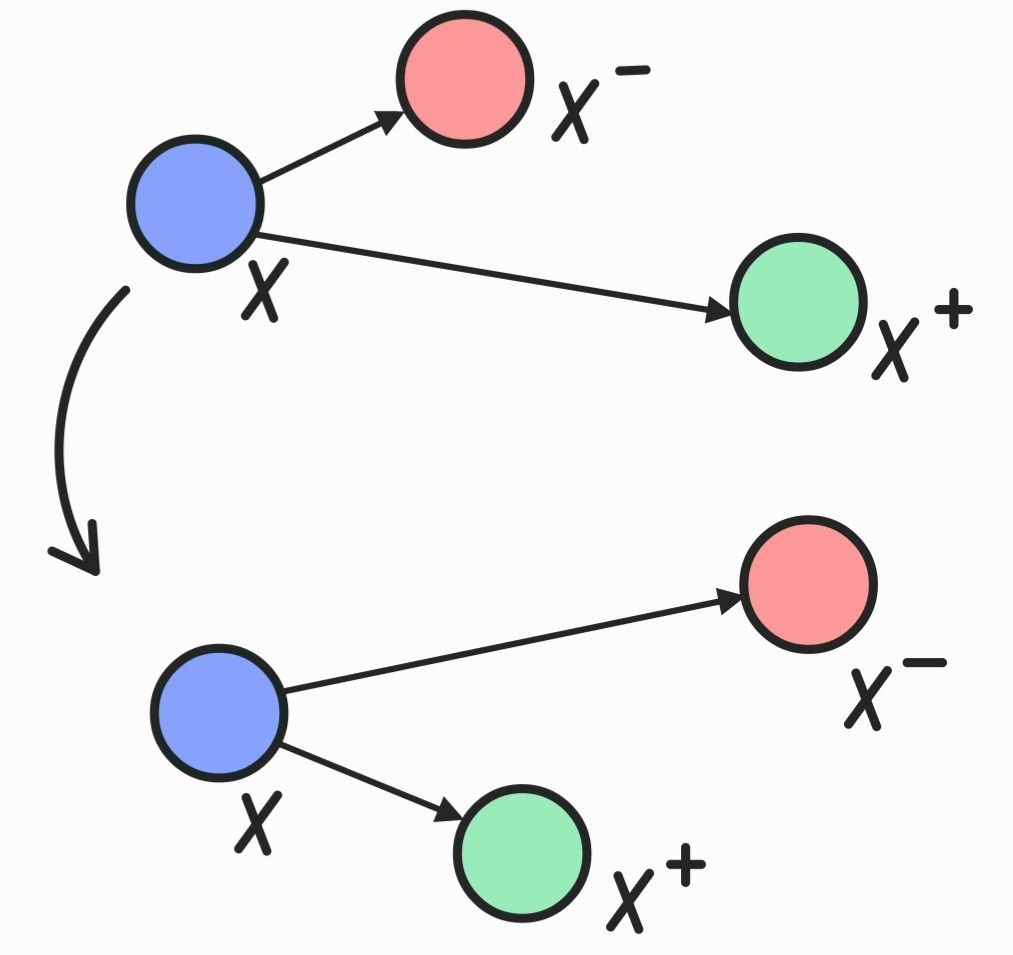
\includegraphics[width=0.3\textwidth]{Presentation/Pictures/Принцип.jpg}
  \end{center}
  \vspace{-20pt}
\end{wrapfigure}

\textit{Обучение сравнениями} – подход при котором обучение происходит посредством попарного сравнения элементов друг с другом.

\bigskip

Пусть $\mathbf{x}$ -- вектор основного объекта. Тогда вектор схожего объекта $\mathbf{x}^+$ -- позитивный элемент. Вектор отличного объекта $\mathbf{x}^-$ -- негативный элемент. $f$ -- модель. Задача обучения сравнениями:

\[\text{dist}(f(\mathbf{x}), f(\mathbf{x}^+)) \to \underset{f}{\min}, ~~~ \text{dist}(f(\mathbf{x}), f(\mathbf{x}^-)) \to \underset{f}{\max}.\]

\bigskip

Так как решается задача обучения без учителя, появляется смещение ввиду неверного сэмплирования. Например, при чрезмерной аугментации положительной пары или при представлении всего батча в качестве негативных элементов.

\[\text{dist}(f(\mathbf{x}), f(\mathbf{x}^+_{\text{wrong}})) \nrightarrow \underset{f}{\min}, ~~~ \text{dist}(f(\mathbf{x}), f(\mathbf{x}^-_{\text{wrong}})) \nrightarrow \underset{f}{\max}.\]
\end{frame}
%----------------------------------------------------------------------------------------------------------
\begin{frame}{Смещение ложноотрицательных элементов}
\small
Классическая функция потерь, не учитывающая смещения:
\[\mathcal{L}_{\text{N-pair}}^N(f) = - \log \frac{\exp(f(\mathbf{x})^T f(\mathbf{x}_i^+))}{\exp(f(\mathbf{x})^T f(\mathbf{x}_i^+)) + \sum _{i=1}^{N} \exp(f(\mathbf{x})^Tf(\mathbf{x}_i^-))}.\]

Устранение смещения ложноотрицательных элементов\footfullcite{Chuang et al., 2020}:

\[p_\mathbf{x}^-(\mathbf{x}') = \frac{p(\mathbf{x}') - \tau^+ p^+_\mathbf{x}(\mathbf{x}')}{\tau^-},\]

\begin{equation*} \small
\mathcal{L}_{\text{Neg}}^{N}(f) = \mathbb{E}_{\substack{\textbf{x} \sim p; \textbf{x}_+ \sim p_x^+,\\ \{\textbf{u}_i\}_{i=1}^N \sim p^N \\ \textbf{v} \sim p_x^+}}  \bigg[ -\log \frac{e^{f(\textbf{x})^T f(\textbf{x}^+)} }{e^{f(\textbf{x})^T f(\textbf{x}^+)} + N g\big(\textbf{x}, \{\textbf{u}_i\}_{i=1}^N, \textbf{v}\big)} \bigg],
\end{equation*}

\begin{equation*} \small
g\big(\textbf{x}, \{\textbf{u}_i\}_{i=1}^N, \textbf{v}\big) = \frac{1}{\tau^-}\bigg(\frac{1}{N} \sum \limits_{i=1}^N e^{f(\textbf{x})^T f(\textbf{u}_i)} - \tau^+ e^{f(\textbf{x})^T f(\textbf{v})}\bigg).
\end{equation*}
\end{frame}
%----------------------------------------------------------------------------------------------------------
\begin{frame}{Смещение ложноположительных элементов}
\small
Выражение для вероятности получить положительных элемент:

\[p_\mathbf{x}^+ (\textbf{x}') = \frac{p(\textbf{x}') - \tau^- p^-_\mathbf{x}(\textbf{x}')}{\tau^+}.\]

\begin{block}{Лемма (Никитина, 2024)}
% \normalfont 
При $N \to \infty$ несмещённая функция потерь стремится к функции потерь, учитывающей наличие ложноположительных элементов:
\end{block}
\begin{equation*}
\begin{split}
\mathcal{L}_{\text{N-pair}}^N(f) = \mathbb{E}_{\substack{\mathbf{x} \sim p \\ \mathbf{x}^+ \sim p_\mathbf{x}^+ \\ \{\mathbf{x}_i^-\}_{i=1}^N \sim {p_\mathbf{x}^-}^N}} \bigg[ - \log \frac{e^{f(\mathbf{x})^T f(\mathbf{x}^+)}}{e^{f(\mathbf{x})^T f(\mathbf{x}^+)} + \sum_{i=1}^N e^{f(\mathbf{x})^T f(\mathbf{x}_i^-)}} \bigg] \overset{N \to \infty}{\longrightarrow} \\
\overset{N \to \infty}{\longrightarrow} \mathbb{E}_{\substack{\mathbf{x} \sim p \\ \mathbf{x}^- \sim p_\mathbf{x}^-}} \bigg[ - \log \frac{R}{R + N \mathbb{E}_{\mathbf{x}^- \sim p_\mathbf{x}^-} e^{f(\mathbf{x})^T f(\mathbf{x}^-)}} \bigg],
\end{split}
\end{equation*}

\noindent где
\[R = \frac{1}{\tau^+} \big(\mathbb{E}_{\mathbf{x}' \sim p} e^{f(\mathbf{x})^T f(\mathbf{x}')} - \tau^- \mathbb{E}_{\mathbf{x}^- \sim p_\mathbf{x}^-} e^{f(\mathbf{x})^T f(\mathbf{x}^-)}\big).\]
\end{frame}
%----------------------------------------------------------------------------------------------------------
\begin{frame}{Смещенная функция потерь}
\small
\begin{equation*}
\tilde{\mathcal{L}}_{\text{Pos}}^N (f) = \mathbb{E}_{\substack{\textbf{x} \sim p \\ \textbf{x}^- \sim p_x^-}} \bigg[ - \log \frac{\color{violet} \mathbb{E}_{\textbf{x}' \sim p} f(\textbf{x}, \textbf{x}') \color{black} - \tau^- \color{blue} \mathbb{E}_{\textbf{x}^- \sim p_x^-} f(\textbf{x}, \textbf{x}_i^-)}{\color{violet} \mathbb{E}_{\textbf{x}' \sim p} f(\textbf{x}, \textbf{x}') \color{black} + \big(N \tau^+ - \tau^-\big) \color{blue} \mathbb{E}_{\textbf{x}^- \sim p_x^-} f(\textbf{x}, \textbf{x}_i^-)}\bigg].
\end{equation*}

Финальная оценка:
\begin{equation*}
\mathcal{L}_{\text{Pos}}^N (f) = \mathbb{E}_{\substack{\textbf{x} \sim p \\ \{\textbf{u}_i\}_{i=1}^N \sim {p_x^-}^N \\ \textbf{v} \sim p_x}} \bigg[-\log \frac{\color{violet}P_{\text{emp}} \color{black} - \tau^- \color{blue} P_{\text{emp}}^-} {\color{violet}P_{\text{emp}} \color{black} + \big(N \tau^+ - \tau^-\big) \color{blue} P_{\text{emp}}^- }\bigg],
\end{equation*}

\noindent где $P_{\text{emp}}$, $P_{\text{emp}}^-$ -- эмпирические оценки матожиданий:

\[P_{\text{emp}} (\textbf{x}, \{\textbf{u}_i\}_{i=1}^N, \textbf{v}) = \frac{1}{N+2} \bigg(\sum \limits_{i=1}^N e^{f(\textbf{x})^T f(\textbf{u}_i)} + e^{f(\textbf{x})^T f(\textbf{v})} + e^{f(\textbf{x})^T f(\textbf{x})}\bigg),\]

\[P_{\text{emp}}^- (\textbf{x}, \{\textbf{u}_i\}_{i=1}^N) = \frac{1}{N} \sum \limits_{i=1}^N e^{f(\textbf{x})^T f(\textbf{u}_i)}.\]
\end{frame}
%----------------------------------------------------------------------------------------------------------
\begin{frame}{Корректность функции потерь для задачи}
\begin{block}{Теорема (Никитина, 2024)}
Задача минимизации $\mathcal{L}_{\text{Pos}}^N$ эквивалентна задаче максимизации совместной информации между положительной парой $I(\mathbf{x}, \mathbf{c})$, то есть:

\[I(\mathbf{x}, \mathbf{c}) = \sum\limits_{\mathbf{x} \in X, \mathbf{c} \in C}p(\mathbf{x}, \mathbf{c})\log \frac{p(\mathbf{x}|\mathbf{c})}{p(\mathbf{x})} \geq\]

\[\geq \mathbb{E}_{\mathbf{x} \sim p}\log\left((N + 2)\frac{p(\mathbf{x}|\mathbf{c})}{p(\mathbf{x})}\right) - \mathcal{L}_{\text{Pos}}^N\]
\end{block}
\end{frame}
%----------------------------------------------------------------------------------------------------------
\begin{frame}{Эксперимент на искусственных данных}
\small
\begin{block}{Цель}
Проверить способность функции потерь $\mathcal{L}_{\text{Pos}}(f)$ восстанавливать начальное распределение.
\end{block}

\begin{block}{Метод}
\[\mathcal{L} = \mathcal{L}^N_{\text{Pos}}(f) + \mathcal{D}_{\text{KL}}(f||\mathcal{N}(\mathbf{0}, \mathbf{I}))\]
\end{block}

\begin{figure}
    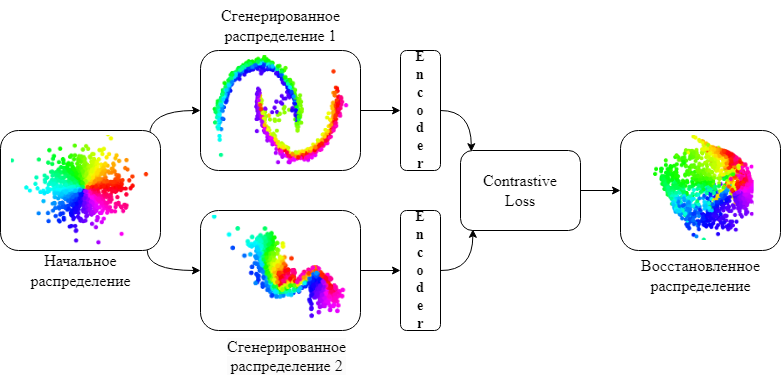
\includegraphics[width=0.9\linewidth]{Presentation/Pictures/Model.png}
\end{figure}
\end{frame}
%----------------------------------------------------------------------------------------------------------
\begin{frame}{Классификация изображений: метод}
\small
\begin{block}{Цель}
Сравнить работу модели с $\mathcal{L}_{\text{N-pair}}(f)$, $\mathcal{L}_{\text{Neg}}(f)$ и $\mathcal{L}_{\text{Pos}}(f)$ на задаче классификации на датасете MNIST10.
\end{block}

\begin{block}{Метод}
\begin{itemize}
    \item $\mathcal{T}$ -- семейство аугментаций.
    \item Семплируются 2 аугментации $t, t' \sim \mathcal{T}$, применяются к каждому объекту.
    \item Обучается сеть-энкодер $f(\cdot)$ и сеть-проекция $g(\cdot)$ для максимизации соответствия представлений.
\end{itemize}
\end{block}

\begin{block}{Метрики}
В качестве метрик берётся Accuracy и Top-k-accuracy:

\[Acc_1 = \frac{TP + TN}{TP + FP + TN + FN}, ~~~ Acc_k = \frac{1}{n}\sum\limits_{i=1}^n[y_i \in \hat{y}_i^k]\]
\end{block}
\end{frame}
%----------------------------------------------------------------------------------------------------------
\begin{frame}{Классификация изображений: результаты}
\begin{table}
\begin{center}
\begin{tabular}{| c | c | c | c |}
\hline
& $\mathcal{L}_{\text{N-pair}}$ & $\mathcal{L}_{\text{Neg}}$ & $\mathcal{L}_{\text{Pos}}$ \\ \hline
Acc1 & 74.84 & 75.81 & \textbf{77.45}\\ \hline
Acc5 & 98.56 & 98.56 & \textbf{98.58}\\ \hline
\end{tabular}
\end{center}
\end{table}

\begin{figure}
   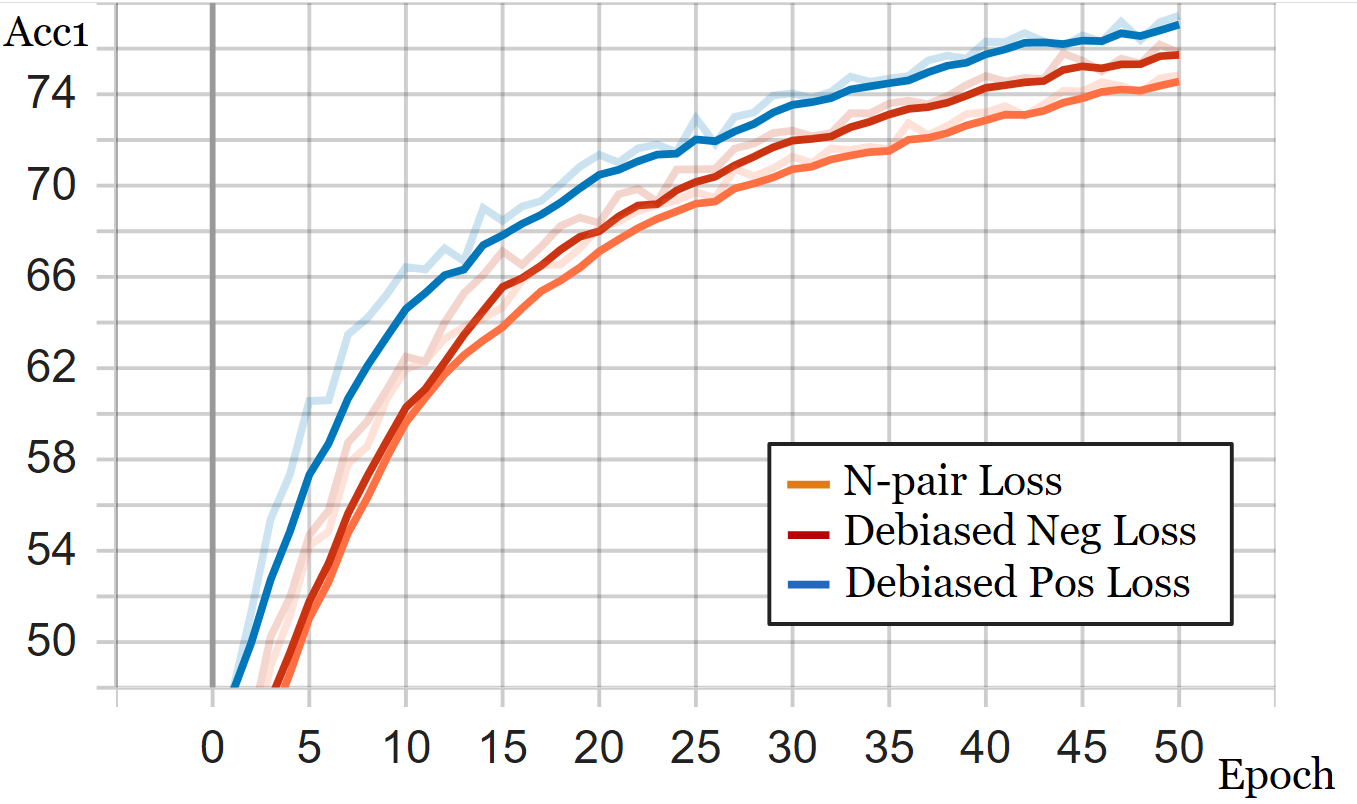
\includegraphics[width=0.475\textwidth]{Presentation/Pictures/loss_acc1_new.png}
   \hfill
   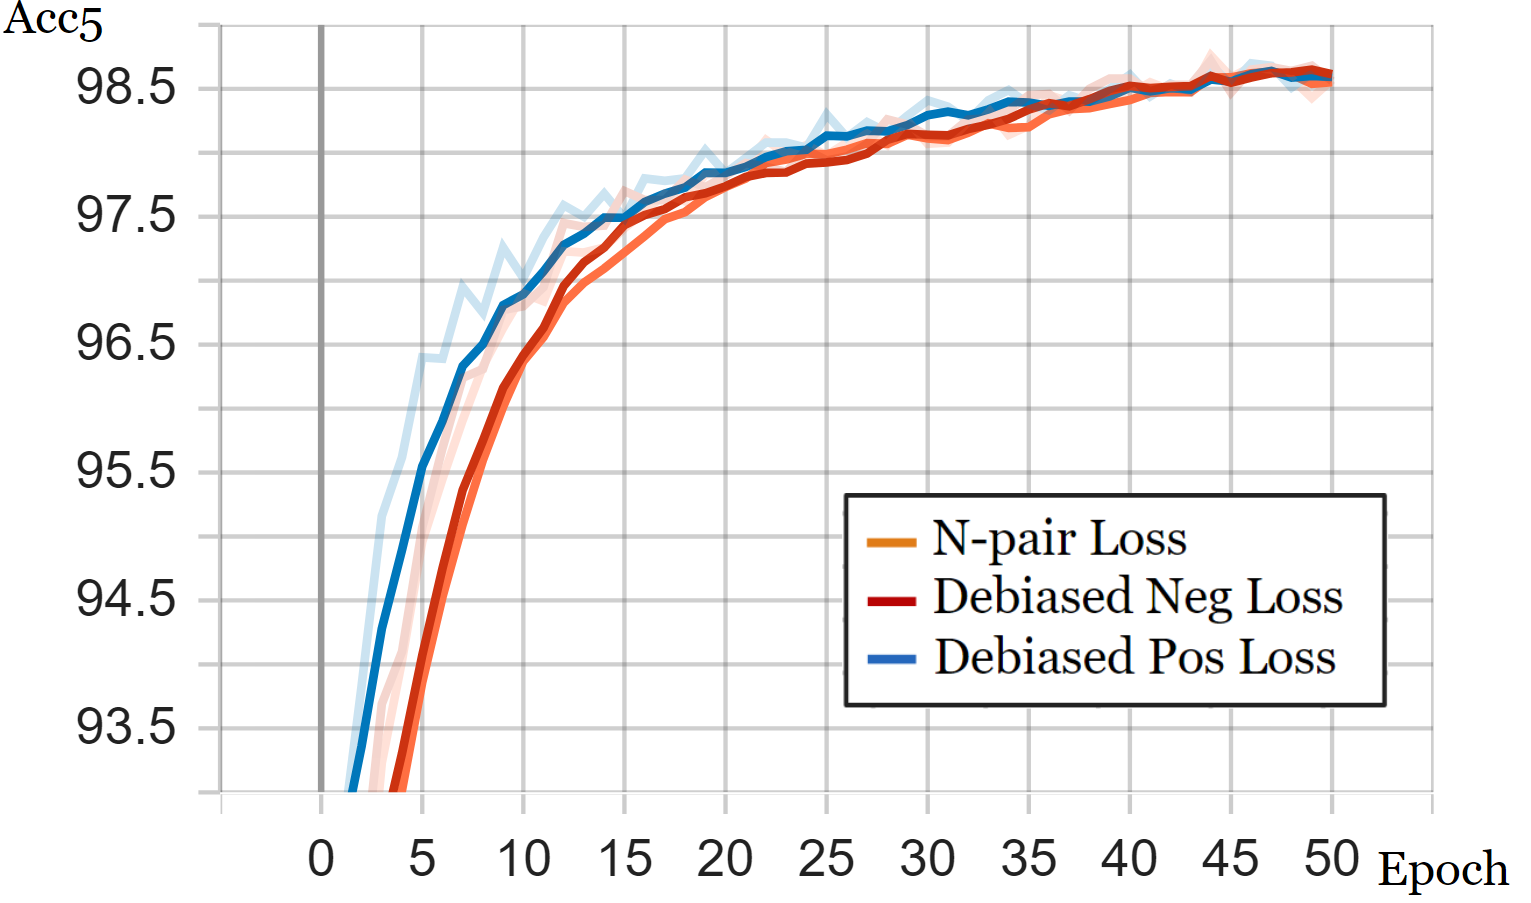
\includegraphics[width=0.475\textwidth]{Presentation/Pictures/loss_acc5_new.png}
\end{figure}
\end{frame}
%----------------------------------------------------------------------------------------------------------
\begin{frame}{Задача ответов на вопросы по изображению}
\scriptsize
\begin{block}{Цель}
Сравнить работу модели с $\mathcal{L}_{\text{Pos}}(f)$ и $\mathcal{L}_{\text{N-pair}}(f)$ на задаче VQA на датасете MS COCO.
\end{block}

\begin{block}{Модель}
В качестве базовой модели берётся TCL\footfullcite{Yang at. al., 2022} с $\mathcal{L}_{\text{N-pair}}$ для сравнений эмбеддингов вида изображение-изображение, изображение-текст, текст-текст. Модель состоит из визуального энкодера  ViT-B/16 и текстового энкодера BERT-base.
\end{block}

\begin{block}{Метрика}
В качестве метрики берётся число попаданий ответа модели в список из 10 ответов, предоставленных авторами датасета:

\[Acc = \frac{1}{n}\sum\limits_{i = 1}^n[y_i \in y_i^{10}]\]
\end{block}

\begin{block}{Результаты VQA для $\mathcal{L}_{\text{N-pair}}$ и $\mathcal{L}_{\text{Pos}}$}
\begin{table}
\begin{center}
\begin{tabular}{| c | c | c |}
\hline
& $\mathcal{L}_{\text{N-pair}}$ & $\mathcal{L}_{\text{Pos}}$ \\ \hline
Accuracy & 66.29 & \textbf{67.23} \\ \hline
\end{tabular}
\label{res_vqa}
\end{center}
\end{table}
\end{block}
\end{frame}
%----------------------------------------------------------------------------------------------------------
\begin{frame}{Пример работы моделей на задаче VQA}
% \begin{figure}
%     \begin{center}
%     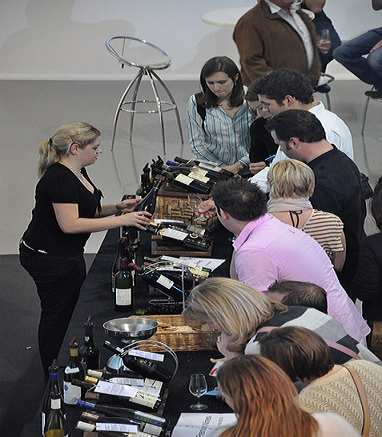
\includegraphics[scale = 0.6]{Presentation/Pictures/image_3.png}
%     \end{center}
% \end{figure}

\begin{columns}
\column{0.5\textwidth}
\begin{figure}
    \centering
    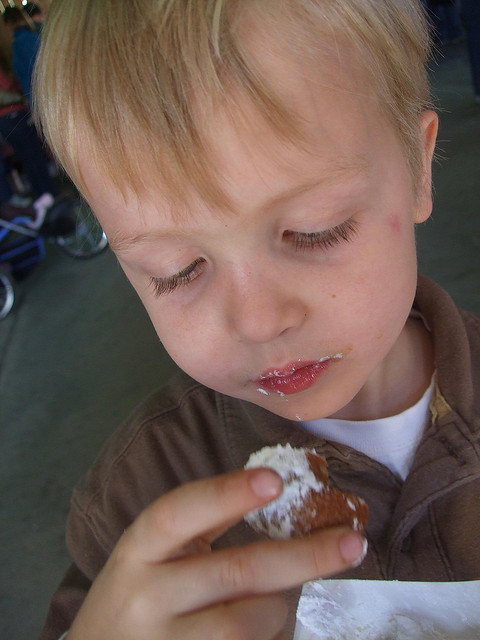
\includegraphics[width=0.8\textwidth]{Presentation/Pictures/contrastive_example.png}
    \caption{Вопрос: «What is the child eating?». Ответ обеих моделей одинаковый и входит в список верных: «donut».}
\end{figure}

\column{0.5\textwidth}
\begin{figure}
    \centering
    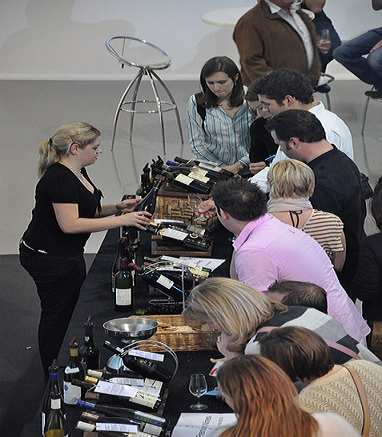
\includegraphics[width=0.8\textwidth]{Presentation/Pictures/image_3.png}
    \caption{Вопрос: «What kind of event are the people involved in?» Ответ модели с $\mathcal{L}_{\text{N-pair}}$: «party» неверный. Ответ модели с $\mathcal{L}_{\text{Pos}}$: «wine testing» входит в список верных.}
\end{figure}
\end{columns}

% Пример работы модели в VQA-задаче. Вопрос: «What kind of event are the people involved in?» Ответ модели с $\mathcal{L}_{N-pair}$: «party» неверный. Ответ модели с $\mathcal{L}_{Pos}$: «wine testing» входит в список верных.
\end{frame}
%----------------------------------------------------------------------------------------------------------
\begin{frame}{Выносится на защиту}
\small
\begin{enumerate}
    \item Исследованы три вида функции потерь в задаче восстановления изначального распределения методом обучения сравнениями: классический N-pair loss и его модификации, устраняющие смещение вследствие наличия ложноположительных и ложноотрицательных элементов выборки.
    \item Предложена функция потерь, устраняющая смещение при ложноположительных элементах. Доказана её сходимость к классическому N-pair loss и свойство максимизации нижней границы взаимной информации.
    \item Проведено сравнение трёх функций потерь в задаче классификации и VQA, а также изучена способность предложенной функции потерь восстанавливать изначальное распределение на примере двумерного пространства.
\end{enumerate}
\end{frame}
%----------------------------------------------------------------------------------------------------------
% \begin{frame}{Список литературы}
% \begin{thebibliography}{99} 
%     \footnotesize
    
%     \bibitem[Chuang, 2020]{p1}
%         Ching-Yao Chuang, Joshua Robinson, Lin Yen-Chen, Antonio Torralba, Stefanie Jegelkah (2020)
%         \newblock Debiased Contrastive Learning

%         \bibitem[Yang, 2022]{p2}
%         Yang, Jinyu and Duan, Jiali and Tran, Son and Xu, Yi and Chanda, Sampath and Chen, Liqun and Zeng, Belinda and Chilimbi, Trishul and Huang, Junzhou (2022)
%         \newblock Vision-Language Pre-Training with Triple Contrastive Learning

%        \bibitem[Chen2020SimCLR, 2020]{p3}
%         CTing Chen, Simon Kornblith, Mohammad Norouzi, Geoffrey Hinton (2020)
%         \newblock A Simple Framework for Contrastive Learning of Visual Representations

%     \bibitem[VQA, 2017]{p4}
%         Stanislaw Antol and Aishwarya Agrawal and Jiasen Lu and Margaret Mitchell and Dhruv Batra and C. Lawrence Zitnick and Devi Parikh (2017)
%         \newblock {VQA}: {V}isual {Q}uestion {A}nswering

%     \bibitem[schroff2015facenet, 2015]{p5}
%         Florian Schroff, Dmitry Kalenichenko, James Philbin (2015)
%         \newblock FaceNet: A Unified Embedding for Face Recognition and Clustering

% \end{thebibliography}
% \end{frame}
\end{document} 